\documentclass[twocolumn]{article}

\usepackage[T2A]{fontenc}
\usepackage[utf8]{inputenc}
\usepackage{amssymb,amsmath,mathrsfs,amsthm}
\usepackage[russian]{babel}
\usepackage{graphicx}
\usepackage{indentfirst}
\usepackage{lipsum}
\usepackage{caption}
\captionsetup{justification=centering}

\usepackage{multicol}
\setlength{\columnsep}{1cm}

\usepackage[style=nature]{biblatex}
\addbibresource{sources.bib}
%\addbibresource{Paper_Ivanov.bib}

\usepackage{geometry}
\geometry{top=25mm}
\geometry{bottom=30mm}
\geometry{left=20mm}
\geometry{right=20mm}

\renewcommand{\baselinestretch}{1.1}
\renewcommand{\baselinestretch}{1.1}

\usepackage{authblk}


\begin{document}

\title{Применение идей фонтанного кодирования\\ при передаче малого числа
битовых пакетов}
\author{Иванов Е.Р.}
\date{\today}

\maketitle
    
\textbf{Аннотация.} В статье изучена возможность
применения идей фонтанного кодирования
при передаче малого числа битовых пакетов:
предложена постановка задачи, допускающая использование
стохастического подхода; предложены
методы ее решения; проведены соответствующие эксперименты
и сделаны выводы о применимости подхода.

\textit{Ключевые слова: теория кодирования, фонтанный код}

\section{Введение}

В конце прошлого века стали активно развиваться технологии,
способные передавать большое количество информации,
например, телевидение и интернет.
Их отличительной чертой также стала не слишком 
высокая цена ошибки декодирования. Именно эти две
особенности процесса передачи информации оказались
решающими в вопросе применимости хорошо изученных 
алгебраических кодов.

Для решения многих задач в новых условиях было бы достаточно, чтобы
ошибки декодирования происходили <<не слишком часто>>
(например, утеря или искажения одного из кадров видеоряда),
а размеры передаваемых битовых последовательностей были
достаточно большими. В качестве решения в начале текущего столетия
были предложены фонтанные коды \cite{MacKay2005Dec, Kythe2017}. В таком случае 
источник работает как
разбрызгивающий пакеты цифровой
фонтан, а для декодирования получателю достаточно лишь собрать в 
<<ведро>> определенное количество
любых «капель».

\section{Постановка задачи}

В качестве модели канала связи использовался BEC (Binary Erasure Channel)
\cite{Kythe2017}. Вероятность утери пакета далее обозначается $\tau$.

Была поставлена следующая задача: используя подходы и идеи 
фонтанного кодирования,
предложить систематический код,
снижающий уровень ошибок в канале
до наперед заданного числа $\pi$ (хорошим результатом
будем считать улучшение на порядок),
используя допустимую избыточность не более $20\%$.
Дополнительным ограничением на течение
процесса является то, что 
количество пакетов, высылаемых при одних и тех же
параметрах, невелико.

Систематичность кода кажется противоречивым 
ограничением для фонтанных кодов, которые были спроектированы 
независящими от порядка посылки символов. Результат, полученный 
М.~Лаби в~\cite{Luby}, сформулирован в предельной форме, в ходе
доказательства встречаются переходы, верные 
при достаточно больших значениях параметров,
поэтому на практике LT-коды оказываются полезными
при значениях $k$ порядка тысяч, что делает их неприменимыми
в поставленной задаче. Однако, можно ослабить одно из
преимуществ фонтанных кодов, заключающееся в независимости
результата от пропускной способности канала связи. Сделаем это, 
дополнительно
предположив, что канал достаточно надежный ($\tau\le7\:\%$),
допустим это как априорное знание.

\section{Изученный подход}

Имеющимися степенями свободы являются алгоритм декодирования
и распределение, по которому
высылаются избыточные пакеты. 
Возможные различные стратегии распределения
сложности между ними. Мы остановились 
на следующем варианте: использование сложного 
алгоритма декодирования -- LT-процесса \cite{Luby} --
и малопараметрического распределения.

Выбор возможных распределений степеней кодирующих символов
осуществлялся исходя из 
следующего наблюдения. 
Удачные распределение идейно выглядят следующим образом:
чаще всего генерируются символы одной и той же степени, которые постепенно
расходуются для поддержания размера очереди.
Перечислим выбранные распределения:

\begin{itemize}

    \item Биномиальное с параметрами $k$ и $p$ 
    \item Пуассоновское с параметром $\lambda$
    \item Степень $d$ с вероятностью 1
    
\end{itemize}

Сделаем несколько замечаний об использовании упомянутых распределений.
В~области значений случайной величины с биномиальным распределением есть ноль, 
что соответствует кодирующему символу нулевой степени; 
с этим недостатком можно, например, бороться с помощью исключения этого значения
и последующей перенормировки, однако в данной работе это
не применялось. Область значений случайной величины с пуассоновским
распределением составляет весь натуральный ряд и ноль; для борьбы 
с возможным символом степени ноль к реализации случайной величины
прибавлялась единица, а в случае равенства значению большего $k$ 
она приравнивалась $k$.

\section{Эксперименты}

Каждый эксперимент однозначно определяется
следующими параметрами: $n$ -- число посылаемых
кодирующих символов, $k$ -- число пакетов, 
$\tau$ -- процент потерь в канале и метод кодирования. 

В качестве оценки $\hat\pi$ для величины $\pi$ -- 
достигнутой пропускной способности канала --  использовалось выборочное 
математическое ожидание:

\[
    \hat\pi = \frac{1}{N_{\mathrm{exps}}}\sum_{j=1}^{N_{\mathrm{exps}}} 
    \left[ 1-
    \frac{N^j_{\mathrm{recovered}}}{k} \right],
\]
где $N_{\mathrm{exps}}$ -- число проведенных экспериментов,
$N_{\mathrm{recovered}}^j$ -- число восстановленных пакетов в $j$ реализации.

Результаты экспериментов приведены на рисунках 
\ref{fig:exp1} и в таблицах 1-2.
По оси абсцисс отложено математическое ожидание
степени каждого кодирующего символа,
по оси ординат -- вычисленная оценка $\hat\pi$.
Запись b в таблице означает, что лучшим оказалось биномиальное распределение,
d -- вырожденное.

\begin{figure*}[ht]
    \centering
    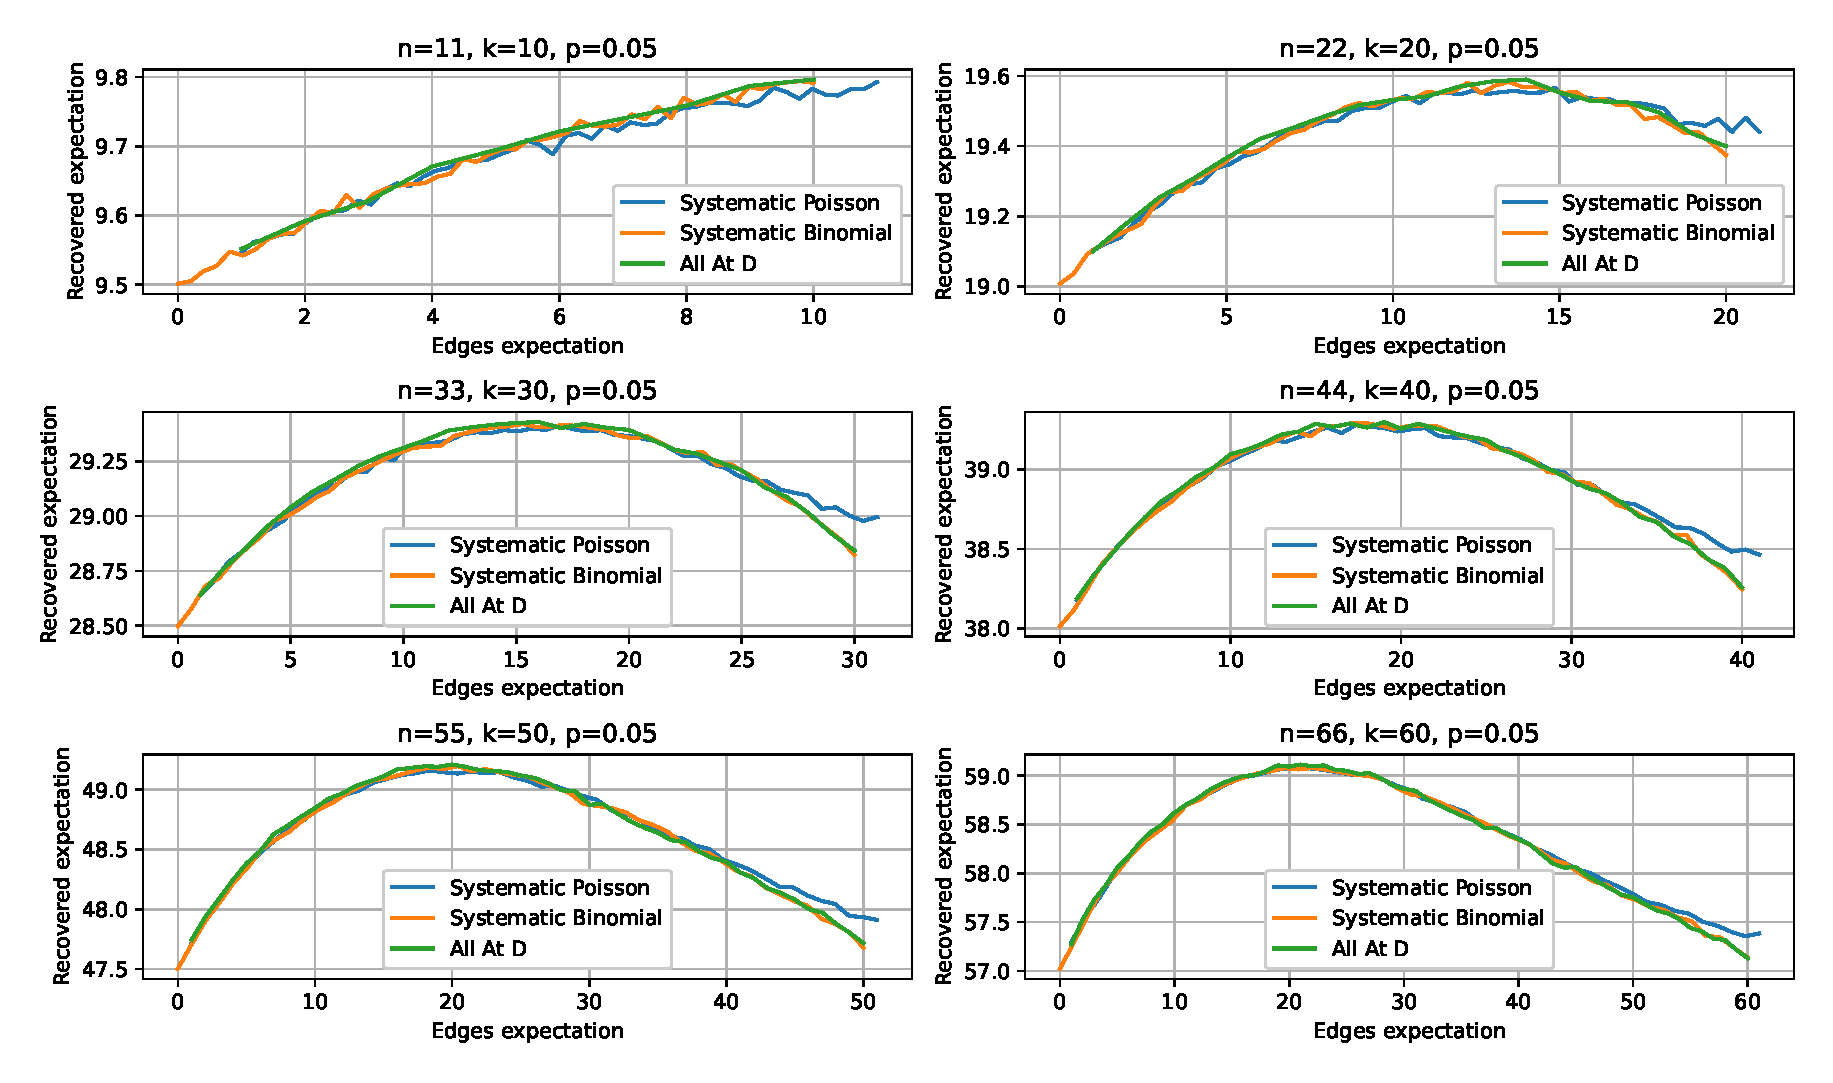
\includegraphics[scale=0.55]{img/exp1.eps}
    \caption{$n=1{,}1k; \tau=0{,}05\%$}
    \label{fig:exp1}
\end{figure*}

\begin{table}
\begin{center}
    \begin{tabular}{|c|c|c|c|}
        \hline
        $n$ & $k$ & Метод & $\hat\pi$ \\
        \hline
        12 & 10 & b & 0{,}0123 \\
        \hline
        24 & 20 & d & 0{,}0083 \\
        \hline
        36 & 30 & d & 0{,}0058 \\
        \hline
        48 & 40 & d & 0{,}0041 \\
        \hline
        60 & 50 & d & 0{,}0030 \\ 
        \hline
        72 & 60 & d & 0{,}0024 \\
        \hline
    \end{tabular}
    \caption{Лучшие результаты методов; $\tau=0{,}05$; избыточность 20\%}
\end{center}
\end{table}

\begin{table}
\begin{center}
    \begin{tabular}{|c|c|c|c|}
        \hline
        $n$ & $k$ & Метод & $\hat\pi$ \\
        \hline
        12 & 10 & d & 0{,}0221 \\
        \hline
        24 & 20 & d & 0{,}0173 \\
        \hline
        36 & 30 & b & 0{,}0132 \\
        \hline
        48 & 40 & d & 0{,}0100 \\
        \hline
        60 & 50 & d & 0{,}0087 \\ 
        \hline
        72 & 60 & d & 0{,}0069 \\
        \hline
    \end{tabular}
    \caption{Лучшие результаты методов; $\tau=0{,}07$; избыточность 20\%}
\end{center}
\end{table}

\section{Выводы}

Опишем сделанные из экспериментов выводы:

\begin{itemize}

    \item для всех распределений верно, что существует
        единственное значение параметра, при котором оно показывает
        наилучший результат;

    \item наиболее удачным оказался опыт использования вырожденного
        распределения (кодирующий символ имеет степень $d$ с вероятностью 1);
        оказалось, что вносимая другими распределениями
        неопределенность в условиях малого количества пакетов скорее мешает, чем помогает;

    \item до максимума значения растут быстрее, чем падают после; это
        объяснимо тем, что при малой средней степени генерируемые пакеты
        скорее неинформативны, так как с большой вероятностью полностью
        <<покрываются>> дошедшими систематическими;

    \item при больших средних значениях степеней лучше работает пуассоновское
        распределение; это объяснимо тем, что оно обладает наибольшей дисперсией,
        а значит при больших средних значениях степеней кодирующие 
        символы меньших степеней будут генеироваться чаще, чем в других
        распределениях.
    
\end{itemize}

\renewcommand{\bibname}{Литература}
\addcontentsline{toc}{section}{\bibname}

\printbibliography[title=Литература]

\end{document}
